\section{Criterio 2: SCREENPLOT DI COTTEL}

Il criterio di Screenplot di Cottel per la selezione dei valori singolari da mantenere della SVD troncata prevede di effettuare un grafico dei valori singolari $\sigma_i$ e di individuare il "gomito" del grafico e mantenere i valori singolari che si trovano prima di esso.\\

\begin{figure}[H]
    \centering
     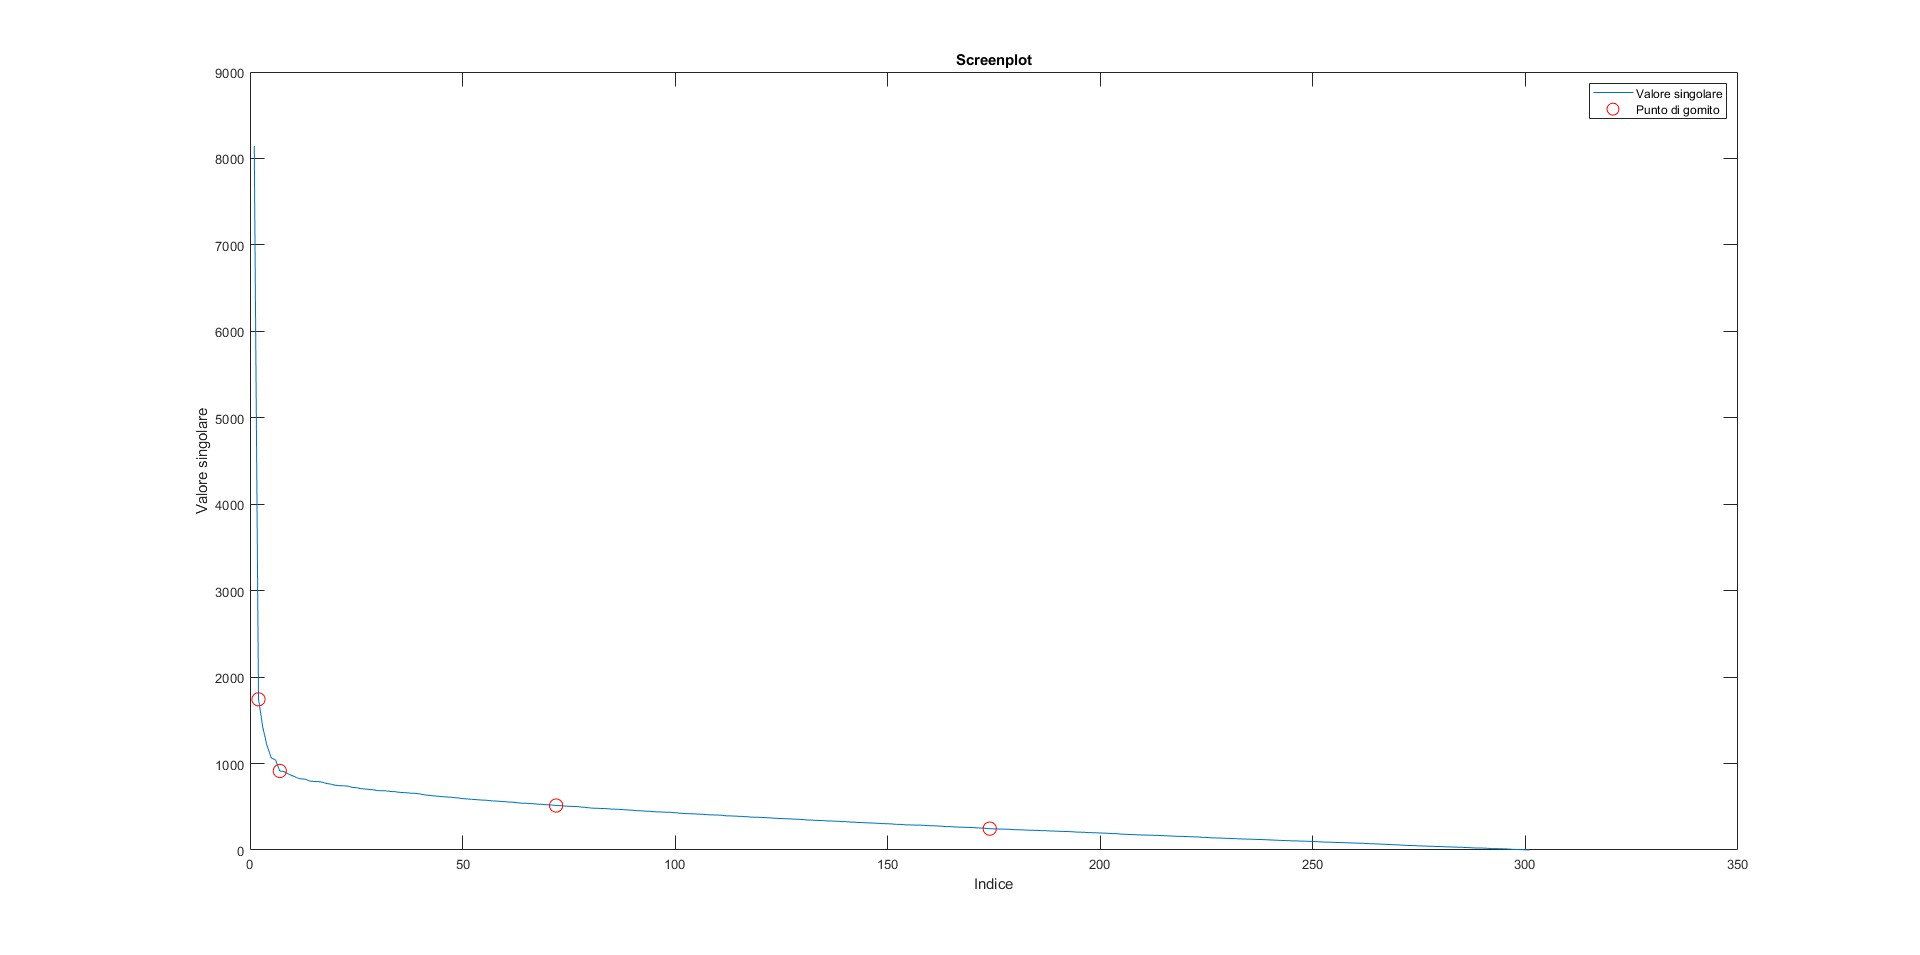
\includegraphics[width=\textwidth]{images/plot.jpg}
    \caption{Plot dei valori singolari}
\end{figure}

\noindent Mediante la funzione \textbf{findchangepts} sono stati individuati 4 punti di gomito. In questo caso si è deciso di procedere con il secondo gomito, ovvero x=7 (di fatto questo criterio è soggettivo).
Sono stati mantenuti i primi 7 valori singolari.\\
\begin{table}[H]
    \centering
    \begin{tabular}{|c|c|c|}
        \hline
        \textbf{Matrice} & \textbf{Righe} & \textbf{Colonne} \\
        \hline
        U\_troncata & 301 & 7 \\
        \hline
        S\_troncata & 7 & 7 \\
        \hline
        V\_troncata & 301 & 7 \\
        \hline
    \end{tabular}
    \caption{Dimensioni matrici troncate}
\end{table}

\begin{table}[H]
    \centering
    \begin{tabular}{|c|c|c|}
        \hline
        \textbf{Norma} & \textbf{Errore assoluto} \\
        \hline
        2 &  907.434068 \\
        \hline
        Frobenius &6782.450233 \\
        \hline
    \end{tabular}
    \caption{Norme ed errori}
\end{table}

\noindent
E' noto inoltre che l'errore assoluto in norma due risulta essere $\sigma_{k+1}$ e in norma Frobenius 
\begin{equation}
    \sqrt{\sum_{i=k+1}^{r}\sigma_i^2}
\end{equation}
 dove k è il numero di valori singolari mantenuti.\\
Per la binarizzazione sono state utilizzate le seguenti soglie:
\begin{itemize}
    \item 0.25
    \item 0.5
    \item 0.75
    \item Soglia automatica calcolata con \textbf{graythresh}
\end{itemize}

\begin{figure}[H]
    \centering
     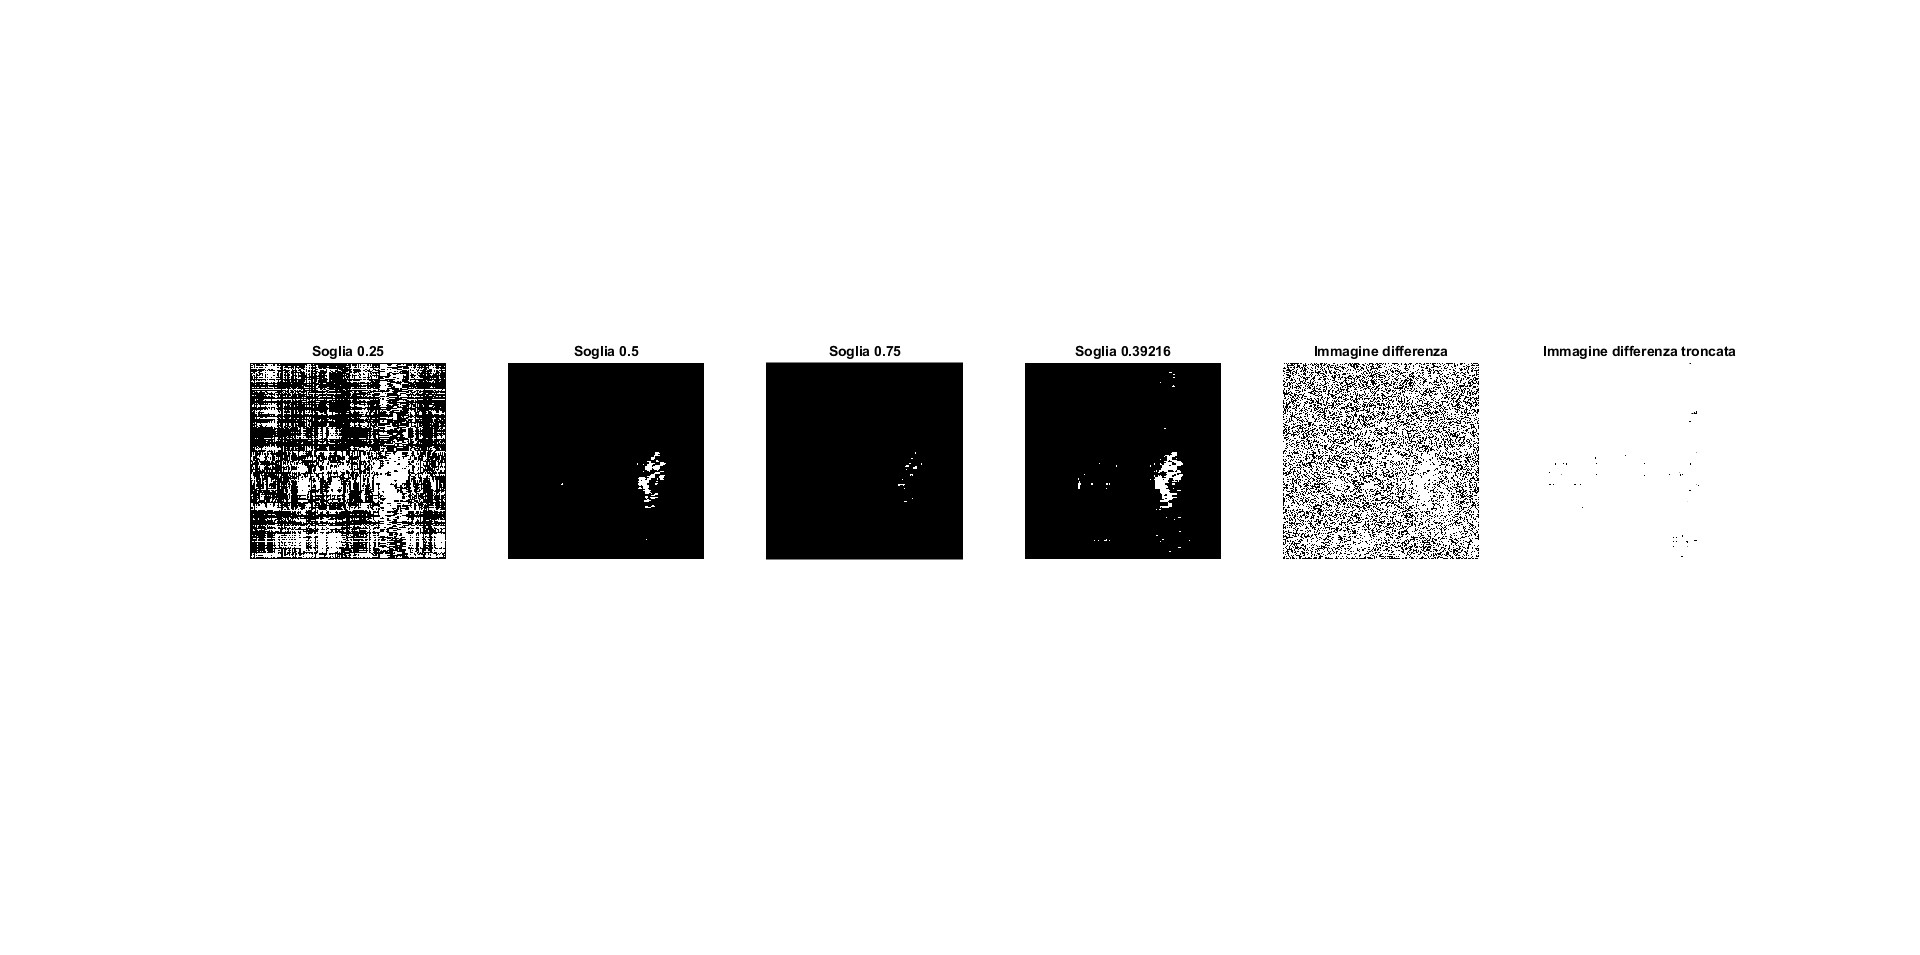
\includegraphics[width=\textwidth]{images/Criterio2.jpg}
    \caption{Immagini binarizzate con criterio 2}
\end{figure}

\noindent Come è possibile notare in questo caso vi è molta differenza tra l'immagine originale e quella approssimata.\\
Osservando le soglie di binarizzazione possiamo vedere come in questo caso la soglia automatica e la soglia 0.5 abbiano prodotto il risultato più "coerente" con l'approssimazione, mentre la soglia 0.25 ha prodotto più "coerente" con l'originale.\\

\noindent Per il processo di troncamento sono stati necessari in media circa \textcolor{blue}{\textbf{0.07}} secondi.\\



